\lab{Изучение плазмы газового разряда в неоне}

%Контрольные вопросы так же стоят после теоретического минимума. В этой лабе и лабе 3.5.2 их не было. Тем не менее, можно в эти лабы добавить вопросы 1, 3--5, 7.

\aim{изучение вольт-амперной характеристики тлеющего разряда; изучение свойств плазмы методом зондовых характеристик.}

\equip{стеклянная газоразрядная трубка, наполненная изотопом неона, высоковольтный источник питания, источник питания
постоянного тока, делитель напряжения, резистор, потенциометр, амперметры, вольтметры, переключатели.}

Схема установки для исследования плазмы газового разряда в неоне представлена на рис.~\figref{Neon gas discharge}. Стеклянная газоразрядная
трубка имеет холодный (ненакаливаемый) полый катод, три анода и \important{геттерный узел}~--- стеклянный баллон, на
внутреннюю поверхность которого напылена газопоглощающая плёнка (\important{геттер}). Трубка наполнена изотопом неона 
$^{22}$Ne при давлении 2~мм~рт. ст. Катод и один из анодов (I или II) с~помощью переключателя $\text{П}_1$ подключаются через
балластный резистор~$R_\text{б}$ ($\sim500$ кОм) к~регулируемому высоковольтному источнику питания (ВИП) с~выходным
напряжением до нескольких киловольт.

\begin{figure}[h!]
	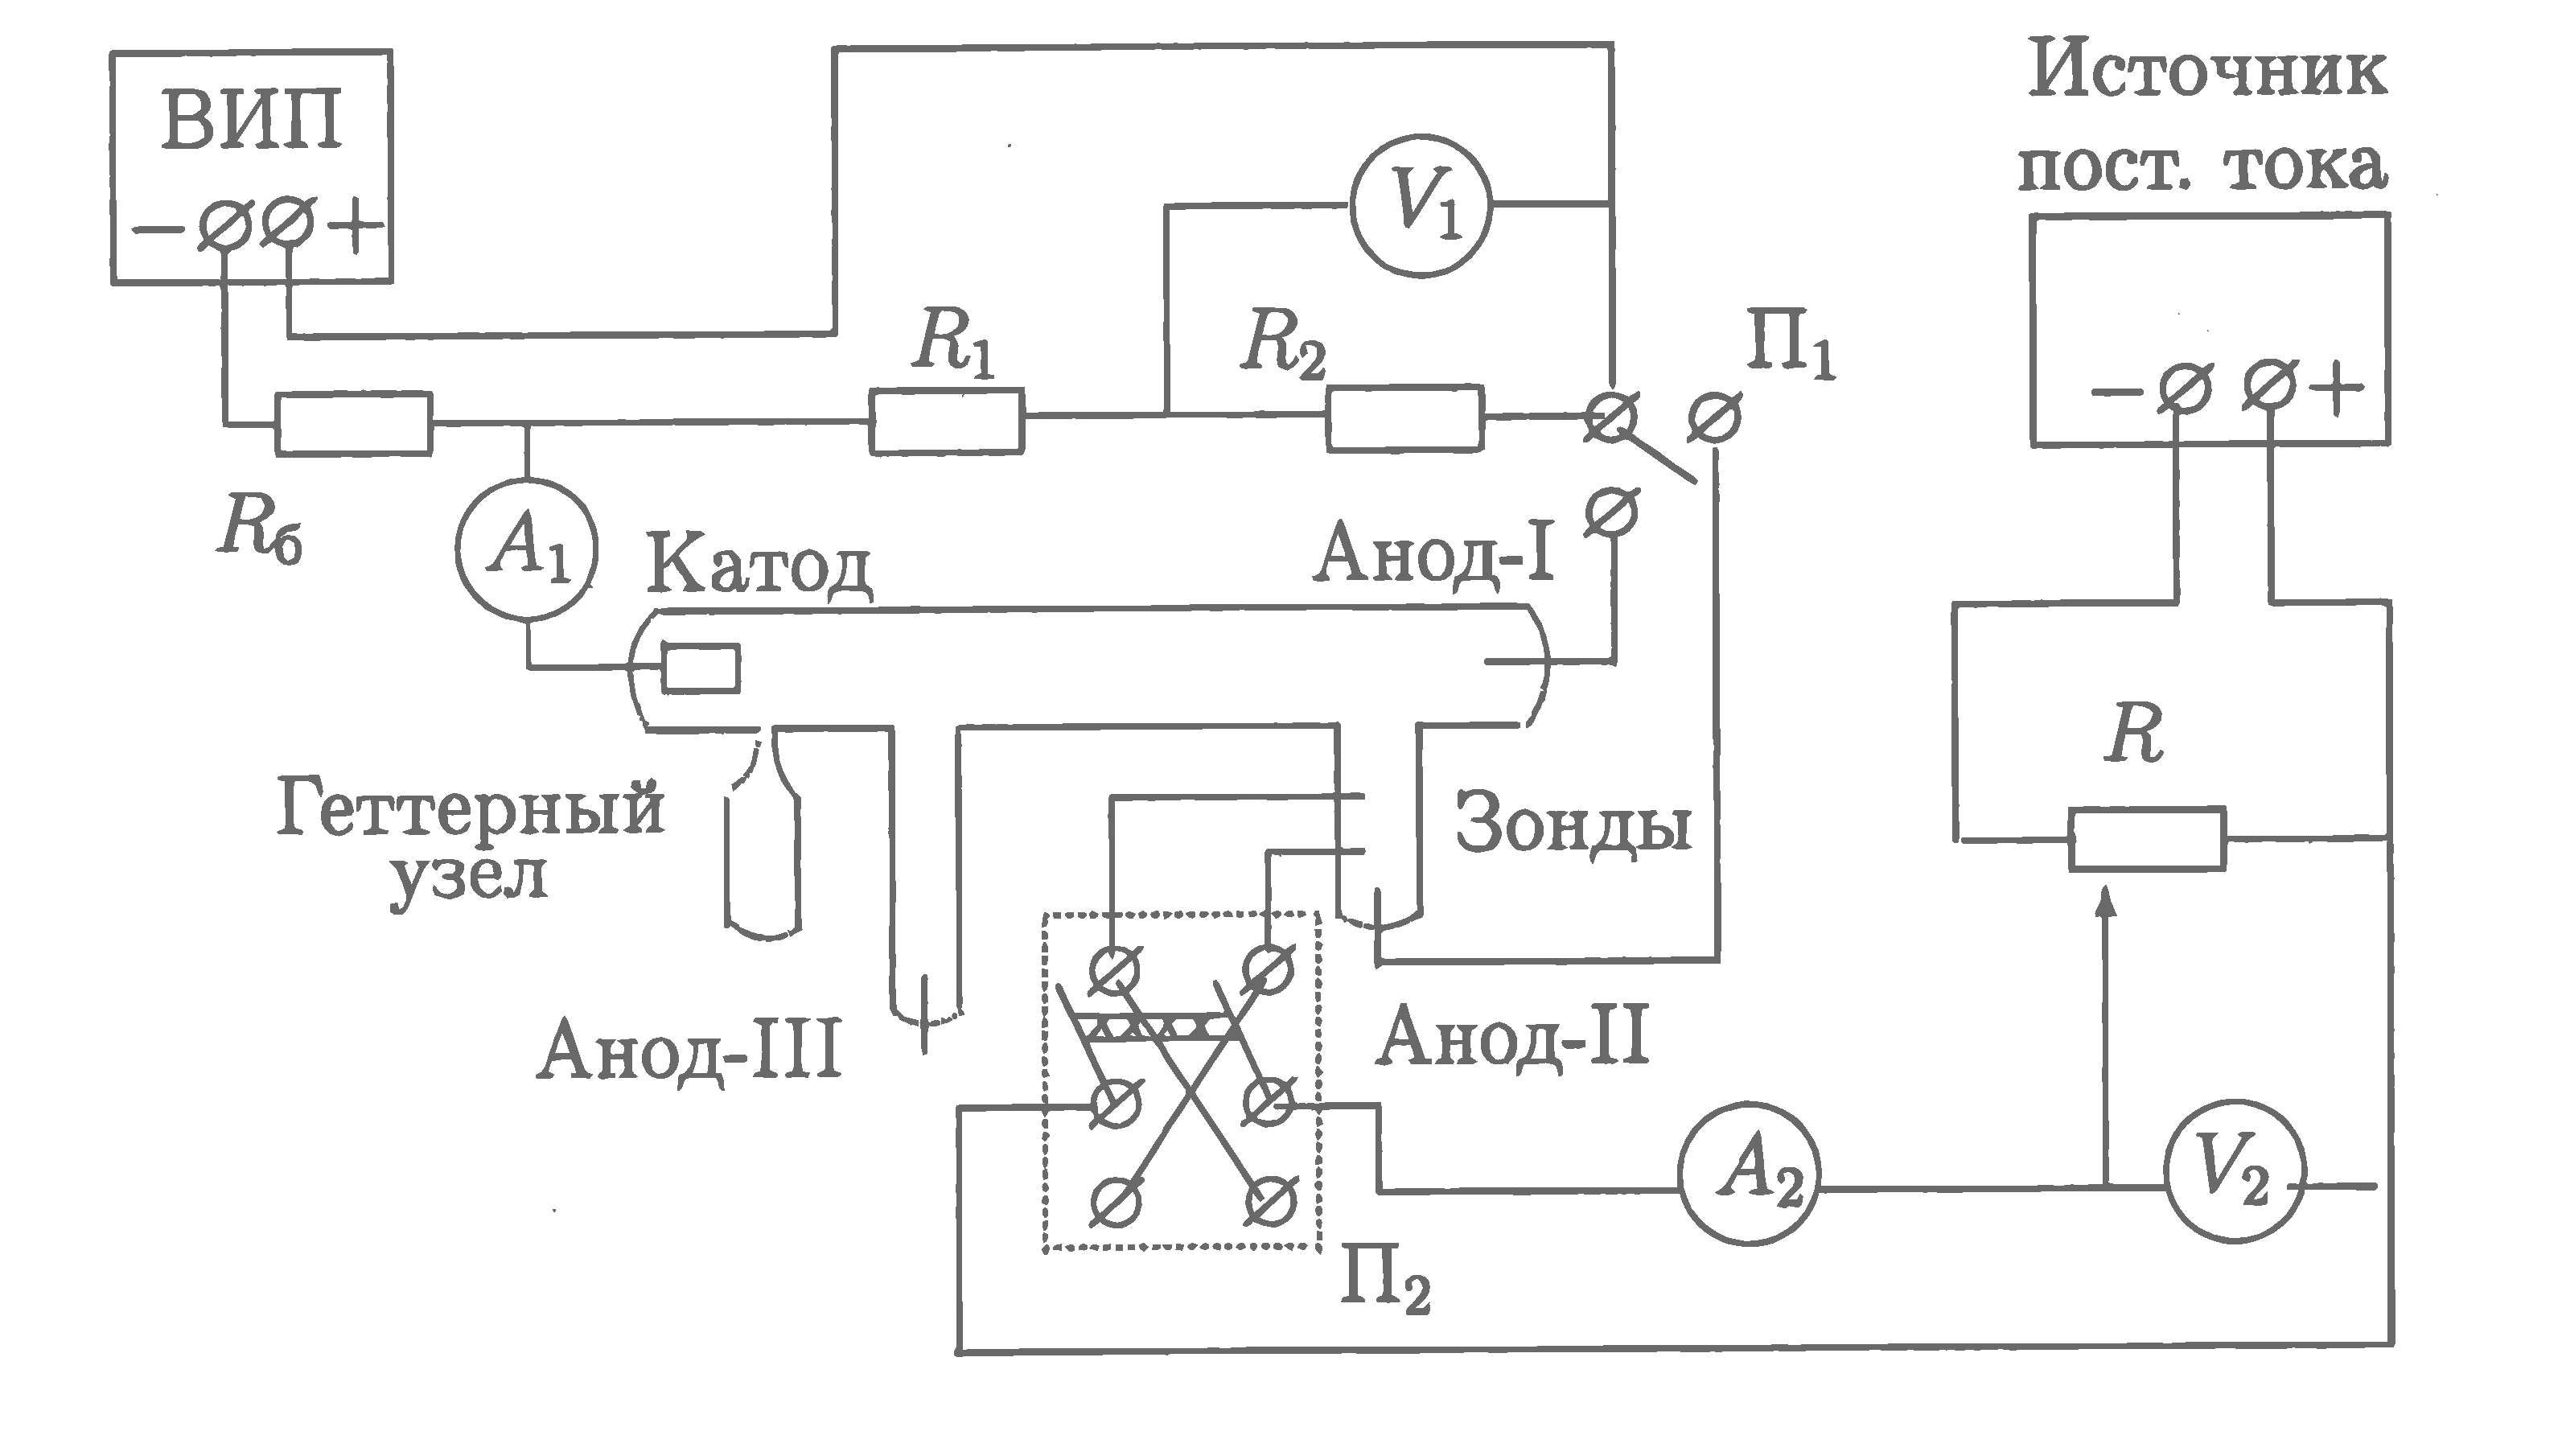
\includegraphics[width = 0.9\textwidth]{Chapter_5/3_5_1.eps}
	\caption{Схема установки для исследования газового разряда}
	\figmark{Neon gas discharge}
\end{figure}

При подключении к ВИП анода-I между ним и катодом возникает газовый разряд. Ток разряда измеряется миллиамперметром
$A_1$, а падение напряжения на разрядной трубке~--- цифровым вольтметром $V_{1}$, подключённым к трубке через
высокоомный (несколько десятков МОм) делитель напряжения с коэффициентом $(R_1+R_2)/R_2$.

При подключении к ВИП анода-II разряд возникает в~проcтранстве между катодом и анодом-II, где находится двойной зонд,
используемый для диагностики плазмы положительного столба. Зонды изготовлены из молибденовой проволоки диаметром
$d$ и имеют длину~$l$. Они подключены к источнику питания через потенциометр~$R$. Переключатель
$\text{П}_2$ позволяет изменять полярность напряжения на зондах. Величина напряжения на зондах изменяется с~помощью дискретного
переключателя <<$V$>> выходного напряжения источника питания и потенциометра $R$, а измеряется вольтметром~$V_2$. Для
измерения зондового тока используется микроамперметр~$A_2$.

Анод-III в нашей работе не используется.


\begin{lab:task}

В работе предлагается снять вольт-амперную характеристику тлеющего разряда и зондовые характеристики при разных токах
разряда и по результатам измерений рассчитать концентрацию и температуру электронов в плазме, степень ионизации,
плазменную частоту и дебаевский радиус экранирования.

 

\tasksection{Вольт-амперная характеристика разряда}

\begin{enumerate}
\item Установите переключатель $\text{П}_1$ в положение <<Анод-I>> и подготовьте приборы к работе согласно техническому описанию, которое находится в лаборатории. Плавно увеличивая выходное напряжение ВИП, определите напряжение зажигания разряда (показания вольтметра $V_{1}$ перед зажиганием). 

\item С помощью вольтметра $V_{1}$ и амперметра $A_{1}$ снимите вольт-амперную характеристику разряда $U_{1}=f(I_\text{р})$. Ток разряда $I_\text{р}$ изменяйте в диапазоне, указанном в описании работы в лаборатории (при больших токах может сгореть сопротивление).

\end{enumerate}

\tasksection{Зондовые характеристики}

\begin{enumerate}
\item Уменьшите напряжение ВИП до нуля, переведите переключатель~$\text{П}_1$
в~положение <<Анод-II>> и подготовьте приборы $\text{П}_{2}$, $V_{2}$ и $A_{2}$ к работе согласно техническому описанию, которое находится в лаборатории. 

\item Плавно увеличивайте напряжение ВИП до возникновения разряда. Установите значение разрядного
тока~$I_\text{р}$ согласно техническому описанию. Подготовьте к работе источник питания. После этого при помощи потенциометра $R$ установите на зонде максимальное напряжение $U_{2 max}$. 

\item Снимите вольт-амперную характеристику двойного зонда $I_{2}=f(U_{2})$ (в диапазоне от $-U_{2 max}$ до $U_{2 max}$) при фиксированном токе $I_\text{p}$ согласно описанию работы в лаборатории.

\item Повторите измерения при другой полярности (переключатель $\text{П}_2$). Менять полярность подключения зондов можно только при \important{нулевом токе}, поддерживая при этом величину тока разряда $I_\text{p}$ в трубке.

Записывая результаты в таблицу, одновременно стройте приближенный график $I=f(U)$  в тетради в интервале от $-U_{2 max}$ до~$U_{2 max}$. Отцентрируйте кривую: проведите ось абсцисс на уровне $I=\sum \Delta I/2$, восстановите ось ординат из точки пересения кривой с новой осью абсцисс. Убедитесь, что можно провести асимптоты к участкам кривой при больших напряжениях. Если точек мало --- проведите дополнительные измерения.

\item Снимите зондовые характеристики при токах разряда, равных 3 и 1,5~мА.
 \end{enumerate}

\tasksection{Обработка результатов}

 \begin{enumerate}

\item Постройте вольт-амперную характеристику разряда $U_{1}=f(I_\text{p})$. По наклону кривой определите максимальное дифференциальное сопротивление разряда $R_{max}$.

\item Постройте семейство зондовых характеристик $I=f(U)$ на одном листе.

\item По зондовым характеристикам определите температуру электронов~$T_{e}$ по формуле \chaptereqref{5.43}: ток $I_{i\text{н}}$ найдите из пересечения асимптоты к току насыщения с осью $U=0$; ($dI/dU)|_{U=0}$~--- наклон
характеристики~$I=f(U)$ в точке $U=0$, $I=0$; взяв $\Delta U$ в вольтах и приняв заряд электрона $e=1$, рассчитайте
энергию (<<температуру>>) электронов ($kT_{e}$) в электрон-вольтах.

\item Полагая концентрацию электронов $n_{e}$ равной концентрации ионов $n_{i}$, определите её из формулы \chaptereqref{5.31}:
\begin{equation}
	I_{i\text{н}}=0,4n_{e}eS\sqrt{\frac{2kT_{e}}{m_{i}}}.
\end{equation}

Здесь $S=\pi\cdot d\cdot l$~--- площадь поверхности зонда; значения $d$ и $l$ приведены в описании экспериментальной
установки; $m_i=22\cdot 1,66\cdot 10^{-24}$~г~--- масса иона неона.

\item Постройте графики $T_e=f(I_p)$, $n_e=f(I_p)$.

\item Рассчитайте плазменную частоту колебаний электронов по формуле:
\begin{equation}
	\omega_{p}=\sqrt{\frac{n_{e} e^2}{\varepsilon_{0} m_{e}} }.
\end{equation}

\item Рассчитайте дебаевский радиус~$r_{D}$ по формуле \chaptereqref{5.18}, которая в случае $T_{e}\gg T_{i}$ принимает в системе СИ вид
\begin{equation}
	r_{D}=\sqrt{\frac{\varepsilon_{0}kT_{i}}{ne^{2}}}.
\end{equation}

\item Оцените среднее число ионов в дебаевской сфере по формуле:
\begin{equation}
	N_{D}=\frac{4\pi}{3} n_{i}r_{D}^{3}.
\end{equation}

\item Оцените степень ионизации плазмы~$\alpha$ (долю ионизованных атомов), если давление в трубке $p\simeq 1$~мбар.

\item Оцените погрешности.

 \end{enumerate}

\end{lab:task}
